
%%%%%%%%%%%%%%%%%%%%%%% file typeinst.tex %%%%%%%%%%%%%%%%%%%%%%%%%
%
% This is the LaTeX source for the instructions to authors using
% the LaTeX document class 'llncs.cls' for contributions to
% the Lecture Notes in Computer Sciences series.
% http://www.springer.com/lncs       Springer Heidelberg 2006/05/04
%
% It may be used as a template for your own input - copy it
% to a new file with a new name and use it as the basis
% for your article.
%
% NB: the document class 'llncs' has its own and detailed documentation, see
% ftp://ftp.springer.de/data/pubftp/pub/tex/latex/llncs/latex2e/llncsdoc.pdf
%
%%%%%%%%%%%%%%%%%%%%%%%%%%%%%%%%%%%%%%%%%%%%%%%%%%%%%%%%%%%%%%%%%%%


\documentclass[runningheads]{llncs}

\usepackage{amssymb}
\usepackage{amsmath}
\usepackage{amsfonts}
\setcounter{tocdepth}{3}
\usepackage{graphicx}
\usepackage{wrapfig}
\usepackage{multirow}
\usepackage{url}

%\urldef{\mailsa}\path|{alfred.hofmann,ursula.barth,ingrid.beyer,natalie.brecht,|
%\urldef{\mailsb}\path|christine.guenther,frank.holzwarth,piamaria.karbach,|
%\urldef{\mailsc}\path|anna.kramer,erika.siebert-cole,lncs}@springer.com|
\newcommand{\keywords}[1]{\par\addvspace\baselineskip
\noindent\keywordname\enspace\ignorespaces#1}
%\renewcommand{\familydefault}{\sfdefault}
%\documentclass{llncs}
%
%\pagestyle{headings}
%\usepackage{amsmath}
\newcommand{\new}{\newcommand}
\new{\bg}{\begin}
\new{\lp}{\left(}
\new{\rp}{\right)}


\newcommand{\xx}{\mathcal{X}}
\newcommand{\yy}{\mathcal{Y}}
\newcommand{\rr}{\mathbb{R}}

\new{\iii}{\begin{enumerate}}
\new{\fff}{\end{enumerate}}
\new{\iiii}{\begin{itemize}}
\new{\ffff}{\end{itemize}}
\new{\mfi}{\begin{eqnarray*}}
\new{\mff}{\end{eqnarray*}}
\new{\mfni}{\begin{eqnarray}}
\new{\mfnf}{\end{eqnarray}}
\new{\beeq}[2]{\begin{equation}\label{#1}{#2}\end{equation}}
\new{\eqn}[1]{~(\ref{#1})}

\new{\room}{\ \ \ \ }
\new{\card}{\#}


\new{\nor}[1]{\|{#1}\|}
\new{\normi}[1]{\left\|{#1}\right\|_{\infty}}
\new{\scal}[2]{\left\langle{#1},{#2}\right\rangle}
\new{\scalh}[2]{\left\langle{#1},{#2}\right\rangle_\hh}
\new{\set}[1]{\{{#1}\}}
% GENERAL MACRO
%%%%%%%%%%%%%%%%%%%%%%%%%%%%
%\new{\rone}{{\mathrm{I\hskip-2.2pt R}}}
\new{\com}{{\mathbb C}}
\new{\rone}{{\mathbb R}} 
\new{\nat}{{\mathbb N}}

\new{\fz}{f_\vz}
\new{\fzlo}{\overline{f}_\vz^\la}
\new{\rd}{\rone^\dm}
\new{\ed}{{\mathbb E}}
%\new{\nat}{{\mathrm{I\hskip-2.2pt N}}}
%\new{\com}{{\mathrm{I\hskip-2.2pt C}}}

%
%\new{\rd}{{\mathrm{I\hskip-2.2pt R}}^\dm}
%\new{\ed}{{\mathrm{I\hskip-2.2pt E}}^\dm}
\new{\argmin}{\operatornamewithlimits{argmin}}
\new{\argmax}{\operatornamewithlimits{argmax}}
\new{\Prob}[1]{\mathrm{P}\left[\, #1 \right]}
\new{\E}{{\mathbb E}}
\new{\eps}{\varepsilon}
%\new{\nor}[1]{\left\|{#1}\right\|}
%\new{\scal}[2]{\left\langle{#1},{#2}\right\rangle}

%LEARNING MACRO
%%%%%%%%%%%%%%%%%%%%%%%%%%%%%
\new{\marg}{\rho_X}
\new{\prob}{\rho}
\new{\dm}{d}
\new{\tr}{\vz}
\new{\n}{n}
\new{\vb}{{\mathbf b}}
\new{\vf}{{\mathbf f}}
\new{\vl}{\bar{\ell}}
\new{\vx}{{\mathbf x}}
\new{\vy}{{\mathbf y}}
\new{\vz}{{\mathbf z}}
\new{\vc}{{\mathbf c}}
\new{\vu}{{\mathbf u}}
\new{\vv}{{\mathbf v}}
%\new{\k}{{\mathcal k}}
%\new{\kx}{{\mathcal k}_x}
\new{\kk}{K}
\new{\s}{K^s}
\new{\kkx}{K_x}
\new{\w}{W}
\new{\wx}{\w_x}
\new{\WW}{{\mathbf W}}
\new{\DD}{{\mathbf D}}
\new{\LL}{{\mathbf L}}
\new{\LS}{{\mathbf L}_{s}}
\new{\LR}{{\mathbf L}_{r}}
\new{\II}{{\mathbf I}}
\new{\KK}{{\mathbf K}}
\new{\ka}{\kappa}
\new{\ls}{\ell}
\new{\err}{{\mathcal E}}
\new{\emp}{{\mathcal E}_z}
\new{\hh}{{\mathcal H}}
\new{\oo}{{\mathcal G}}
\new{\ff}{{\mathcal F}}
\new{\ldue}{L^2(X,\rho)}
\new{\la}{\lambda}
\new{\dd}{\delta}
\new{\vG}{{\mathbf \Gamma}}
\new{\vC}{{\mathbf C}}
\new{\vS}{{\mathbf S}}
\new{\vU}{{\mathbf U}}
\new{\vY}{{\mathbf Y}}
\new{\vX}{{\mathbf X}}
\new{\vaa}{{\boldsymbol{\alpha}}}
\new{\bh}{{\mathcal B}(\hh)}
\new{\hs}{ HS(\hh)}

\new{\lduew}{L^2(X,\rho_\w)}
\new{\Tt}{L_{K,\hh}}
\new{\Tn}{L_{K,n}}
\new{\U}{U_\w}
\new{\LK}{L_{K}}

\new{\Wt}{L_{\w,\hh}}
\new{\Wn}{L_{\w,n}}

\new{\Ah}{A_{\hh}}
\new{\An}{A_{n}}

\new{\Ls}{L_{s}}
\new{\Lr}{L_{r}}

\new{\Lshn}{L_{s,\hh,n}}
\new{\Lrhn}{L_{r,\hh,n}}
\new{\LLsh}{L_{s,\hh}}
\new{\LLrh}{L_{r,\hh}}
\new{\I}{I_{\kk,\w}}
\new{\Ik}{I_\kk}
\new{\IIk}{I^*_\kk}
\new{\Iw}{I_\w}
\new{\IIw}{I^*_\w}

\new{\m}{m}
\new{\mn}{m_{n}}

\new{\Ax}{{A_{\mathbf x}}}
\new{\A}{A}
\new{\AR}{\A^\la}
\new{\ARx}{\A^\la}
%\new{\Tx}{{T_{\mathbf x}}}
\new{\Tx}{L_{K,n}}
%\new{\Sx}{{S_{\mathbf x}}}
\new{\Sx}{{S_n}}
\new{\T}{T}
\new{\Kx}{{K_{\mathbf x}}}
\new{\K}{K}
\new{\g}{{\mathcal G}}
\new{\sn}{\hat{\sigma}}
\new{\vn}{\hat{v}}
\new{\un}{\hat{u}}

\new{\so}{{s^\prime}}

\new{\Pj}{P_j}
\new{\Qj}{Q_j}
\new{\Pnj}{\hat{P}_j}
\new{\Qnj}{\hat{Q}_j}

\new{\cl}{c}
\new{\br}{b}
\new{\R}{R}
\new{\vre}{\vf_\rho}
\new{\re}{f_\rho}
\new{\X}{\mathcal X}
\new{\Y}{\mathcal Y}
\new{\W}{\mathcal W}

\new{\bbeta}{\boldsymbol{\beta}}
%END  command MACRO----------------------------------



\begin{document}

\mainmatter  % start of an individual contribution

% first the title is needed
\title{Towards a theoretical framework for learning multi-modal patterns for embodied agents}

% a short form should be given in case it is too long for the running head
% \titlerunning{Lecture Notes in Computer Science: Authors' Instructions}

% the name(s) of the author(s) follow(s) next
%
% NB: Chinese authors should write their first names(s) in front of
% their surnames. This ensures that the names appear correctly in
% the running heads and the author index.
%
% \author{...%
% \and ...\and ...\and ...}

%%%Authors:
%%%Name	Country	Affiliation	 
%%%Nicoletta Noceti	Italy	Disi	
%%%Barbara Caputo	Switzerland	IDIAP Research Institute	
%%%Claudio Castellini	Italy	University of Genova	 
%%%Luca Baldassarre	Italy	DIFI/DISI - Universita di Genova	 
%%%Annalisa Barla	Italy	DISI - University of Genova	 
%%%Lorenzo Rosasco	United States	MIT	 
%%%Francesca Odone	Italy	DISI	 
%%%Giulio Sandini	Italy	Robotics, brain and cognitive sciences dept - IIT /DIST - Universita di Genova


\author{N.~Noceti$^1$ \and B.~Caputo$^2$ \and C.~Castellini$^3$
\and L.~Baldassarre$^{1,4}$ \and A.~Barla$^1$ \and L.~Rosasco$^{1,5}$ \and
F.~Odone$^1$ \and G.~Sandini$^{3,6}$}
%
% \authorrunning{Lecture Notes in Computer Science: Authors' Instructions}
% (feature abused for this document to repeat the title also on left hand pages)

% the affiliations are given next; don't give your e-mail address
% unless you accept that it will be published
 \institute{
1 - DISI - University of Genova, 
2 - IDIAP - Martigny,\\
3 - DIST - University of Genova,
4 - DIFI - University of Genova,\\
5 - MIT, Cambridge, MA,
6 - IIT, Genova
\\
\vskip 0.3cm
{\tt \{noceti, baldassarre, barla, odone\}@disi.unige.it},\\
{\tt bcaputo@idiap.ch},
{\tt claudio.castellini@unige.it},\\
{\tt lrosasco@mit.edu},
{\tt giulio.sandini@iit.it}
% mail...\\
%\mailsa\\
% \mailsb\\
% \mailsc\\
% \url{...}
 }

%\institute{AFFILIATIONS}
%
% NB: a more complex sample for affiliations and the mapping to the
% corresponding authors can be found in the file "llncs.dem"
% (search for the string "\mainmatter" where a contribution starts).
% "llncs.dem" accompanies the document class "llncs.cls".
%

% \toctitle{Lecture Notes in Computer Science}
% \tocauthor{Authors' Instructions}
\maketitle


\begin{abstract}
% The abstract should summarize the contents of the paper and should
% contain at least 70 and at most 150 words. It should be written using the
% \emph{abstract} environment.

Multi-modality is a fundamental feature that characterizes biological systems 
and lets them achieve high robustness in understanding skills while coping with
uncertainty.
Relatively recent studies showed that multi-modal learning
is a potentially effective add-on to artificial systems, allowing
the transfer of information from one modality to another.
In this paper we propose a general architecture for jointly learning visual and motion patterns: 
by means of regression theory we model a mapping between the two sensorial modalities improving 
the performance of artificial perceptive systems.
We present promising results on a case study of grasp classification in a controlled setting
and discuss future developments. 

\keywords{ multi-modality, visual and sensor-motor patterns, regression theory, behavioural model, objects and actions recognition 
% We would like to encourage you to list your keywords within
% the abstract section
}
\end{abstract}

%\input{introduction_claudio.tex}

 Consider Figure \ref{fig:chairs}, representing $(a)$ a chair, and $(b)$ Santiago
Calatrava's ``sedia redonda'', the round chair, a particularly stylish object of
design sold as a chair in the Sixties. What makes us claim that these objects
both belong to the category of chairs? Indeed, this is an ominous problem in
object recognition: too often the category of an object is determined by its
function rather than by its visual appearance alone. The very concept of object
has been re-defined by Gibson \cite{gibson} in terms of its affordances ---
``what one can do with it''. According to this view, what ties both the objects in
Figure \ref{fig:chairs} to the category of chairs is the fact that they are
used to sit down.

Further hints at a strong link between perception and action come from neuroscience,
in particular from the mirror neurons paradigm \cite{fadiga}. According to the
mirror theory, neural correlates are found for both the performance of a grasping
action (mainly involving the sensorimotor system of primates) and its visual
representation when performed by another primate (involving the visual system only).
If this is true, as it seems, then the monkeys' (and our) object classification is
so robust mainly because these biological systems \emph{know what to do} with the
objects they see --- a capability which machines lack, so far. Picture, for instance,
how much easier automated object recognition of a mug would be under changing illumination
conditions, if only our machine had an idea of how to grasp something which looked like
a mug.

Inspired by these considerations, we hereby define a theoretical framework for
reconstructing \emph{active} sensory modalities from \emph{passive} ones, that is in
short, for figuring out what to do with what one sees, hears, smells etc. In particular,
we enforce one such schema using a multi-variate regression technique to associate
\emph{object visual features} to related \emph{human grasping postures}. This schema is
called a \emph{Visuo-Motor Map} (VMM) and is trained
using a large database of visual and motor data collected from human subjects, that
we call the \emph{Visuo-Motor Grasping dataBase} (VMGdB). The immediate result is the
ability of retrieving a (set of) grasping posture(s) just by seeing an object; this
ability, which we call \emph{grasp priming}, has obvious applications in robotic fields
where (semi)autonomous grasping / fine manipulation is reuquired, such as robotic surgery,
humanoid robotics, teleoperation, advanced hand prosthetics etc.

Since, though, the focus of this work is on enhancing object reocgnition, we then show
that these grasping postures, reconstructed by the VMM, dramatically improve the
classification rate of a standard object classifier.

The paper is organised like this: in Section \ref{sec::framework} we define the general
multi-modal learning framework, and then we describe the instance under examination;
we then describe in detail the vision-related unit (Section \ref{sec::vision}) and the
regression schema employed to build the VMM (Section \ref{sec::regression}). We then show our
experimental results (Section \ref{sec::experiments}) and conclude in Section \ref{sec::concl}.

%\begin{itemize}
%
%\item learning by imitation great capability of cognitive systems. It permits to learn how to grasp a cup never seen before just by seeing someone else doing it.
%Fundamental learning mechanism etc 
%
%\item a widely accredited hip is that the underlying mechanism of learning by imitation is the existence of a sensor motor map that links
%the visual perception of an object to the motir position of the hand when it manipulates it. Mirror neurons blabla 
%
%\item another consequence of the existence of a sensor-motor map is that when we learn an object by seeing and manipulating it, we are then able
%to recognize it with a higher degree of accuracy and robustness than if we would have learned it on visual data only. 
%
%\item Enabling a robot to display similar abilities is one of the holy grails of research in artificial cognitive systems. 
%
%\item In this paper we present a mirror neurons inspired algorithm for building perception action maps between visual, passive perception and motor, active
%perception. During learning, the algorithm takes as input visual and sensomotor data and (a) it builds a mapping between the two modalities (b) it builds 
%a classifier on both modalities. After training, wehn presented with a visual input, the system is able to perform grasp priming (= is able to predict
%which are the possible way to grasp the seen object; this information could be used to pre-activate a robot hand) and enhanced visual recognition
%(= is able to recognize objects with a higher degree of accuracy and robustness compared to a model learned only on visual features, even if
%the sensor modality is not perceived by the agent). Experiments show that.....
%
%\item in the rest of the paper...
%
%\end{itemize}


\section{A theoretical framework for multi-modal learning}
\label{sec::framework}

As outlined in the Introduction, we assume that there exists a mapping between (sets of) patterns belonging to different modalities --- here we focus upon the relations which exist between a passive and an active modality. In the aforementioned example dealing with objects (as seen) and grasping them, something like what is shown in Figure \ref{fig::implementation} is sought for.

\begin{figure}[h!]
	\centering
	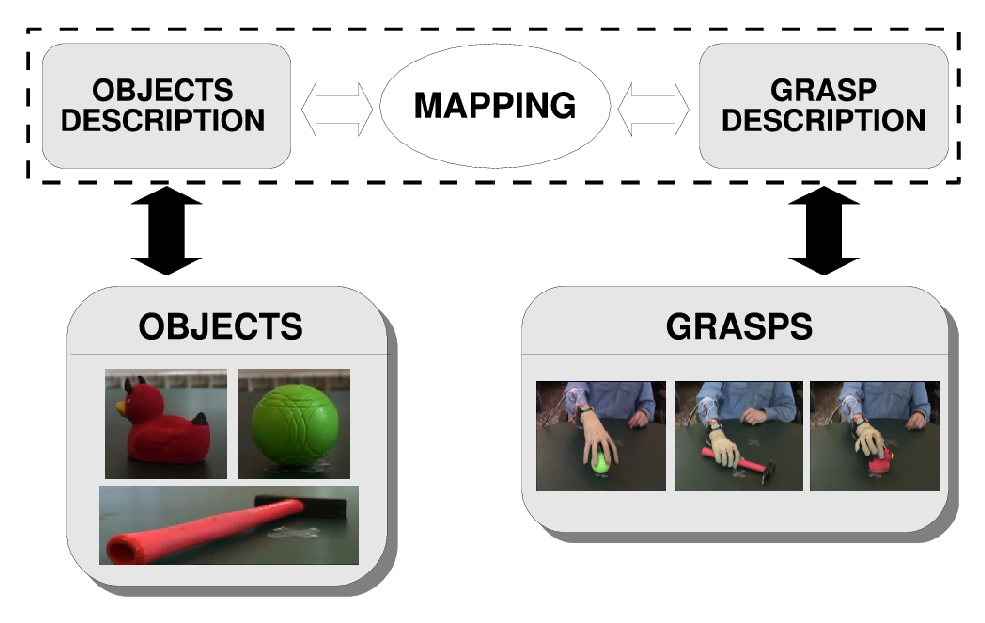
\includegraphics[width=0.7\textwidth]{images/schema_implementazione}
	\caption{An instance of the framework we propose: estimating a
     mapping between appropriate visual descriptions of objects and
     classes of grasp actions. For the time being, we assume that such
     relation is a one-to-one mapping.}
	\label{fig::implementation}
\end{figure}
%\vskip -0.5cm

In general, active modalities are not available to a biological system during the prediction phase, but only during the training phase. A paradigmatic example is that of a human infant learning how to grasp an object: by repeatedly trying to apply, e.g., a cylindric grasp to a bottle, he will learn not only to do it more and more efficiently, but also that a bottle is better be grasped cylindrically when moving it or bringing it close to the mouth. Later on, the sight of a bottle will remind the young human what one of the correct grasps is for that particular object. 
A \emph{perception-to-action map} (PAM) is the equivalent of such training for a biological system: a model to reconstruct an active modality from a passive one. The PAM of our example is a mapping from visual features of an object to motor features of the grasping action used for that object. In general such a map is many-to-many: both a hammer and a bottle can be grasped cylindrically\footnote{the nomenclature of grasp types loosely follows that of Cutkosky \cite{cutkosky}.}), and as well a mug can be handled either cylindrically or by the handle. In this work we make the simplifying assumption that for a specific object there is just one acceptable grasping action --- the PAM is one-to-one.
A PAM is useful in passive pattern recognition (e.g., classifying an object just by seeing it) since it augments the input space with PAM-reconstructed active patterns (e.g., classifying the same object from its sight \emph{and the associated grasp}). In this preliminary work we focus upon a simpler problem, namely that of checking whether, given the visual features of an object, the PAM-reconstructed grasp is (similar to) the one associated with that particular object. For example, we might train a PAM to reconstruct a pinch grip (hand posture) from the visual features of a pen; given then, in the prediciton phase, the visual features of another pen, will the PAM-reconstructed hand posture of a pinch grip look like a true pinch grip?

% We consider $5$ grasp types, shown in Figure \ref{fig::grasps}, identified by different hand postures.

% \begin{figure}
% 	\centering
% 	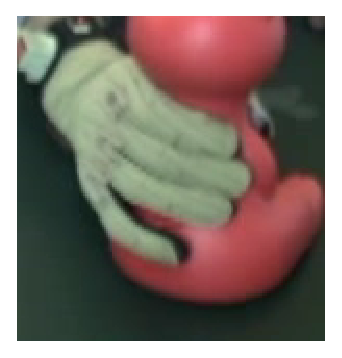
\includegraphics[width=0.19\textwidth]{images/cylinder}
% 	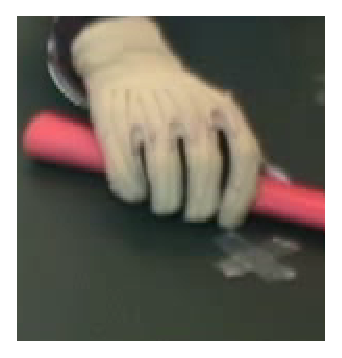
\includegraphics[width=0.19\textwidth]{images/flat}
% 	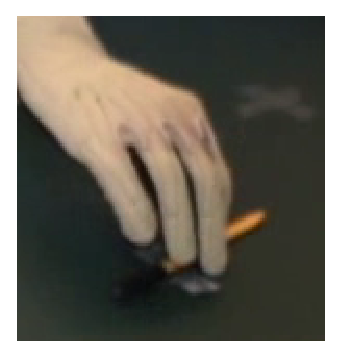
\includegraphics[width=0.19\textwidth]{images/pinch}
% 	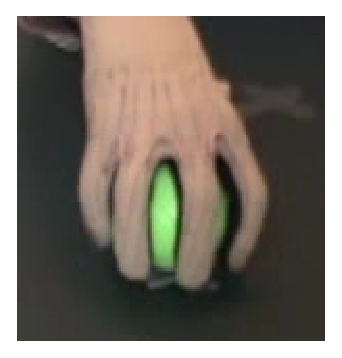
\includegraphics[width=0.19\textwidth]{images/spherical}
% 	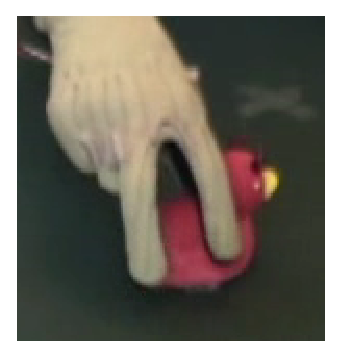
\includegraphics[width=0.19\textwidth]{images/tripodal}
% 	\caption{The grasp types considered in this work: \emph{(left to right)}
% 	   cylindric power grasp, flat grasp, pinch grip, spherical and
% 	   tripodal grip.}
% 	\label{fig::grasps}
% \end{figure}

In particular, what is needed is: $(i)$ a \emph{vision unit} to extract visual features from an image or a series of images, and $(ii)$ a \emph{regression unit}, which will build the PAM.
%Notice that, given our assumption that this PAM is one-to-one, a simple regression method can be used to build it, i.e., we don't have to resort to probabilistic methods such as, e.g., mixture density networks, as it has been done in literature \cite{richmond}.

%Among the various issues and possible applications taking shape from the general schema described so far, the problem we are interested to face can be stated as follows: supposing that it exists a relation between objects and actions, are we able to model it? Our idea is to exploit such relation to obtain joint information about object and action, that is predicting one of them given the other.\\
%\begin{figure}
%	\centering
%	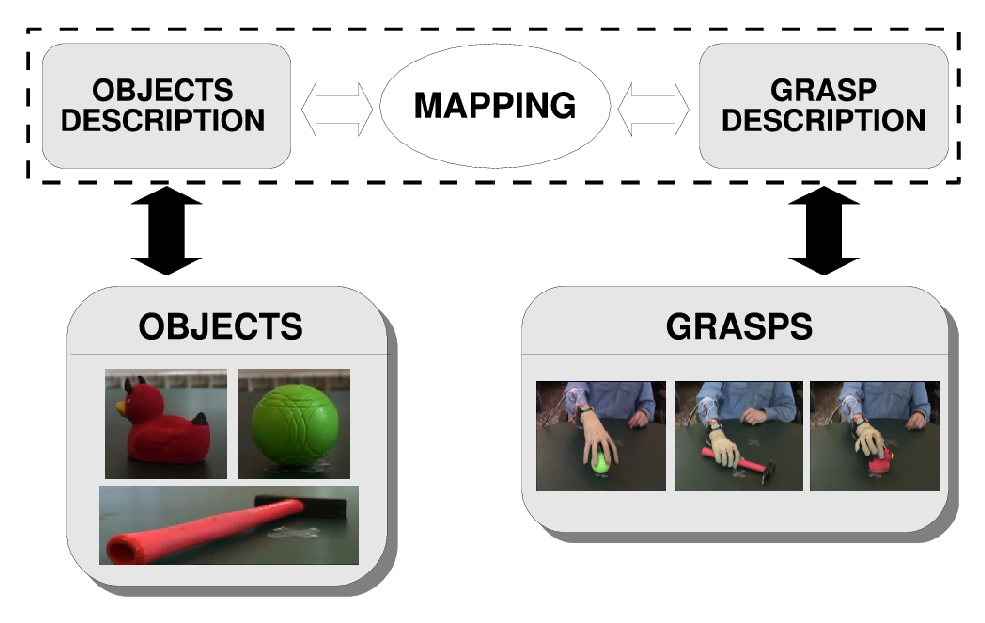
\includegraphics[width=0.7\textwidth]{images/schema_implementazione}
%	\caption{The implementation that we consider relies on estimating a mapping between appropriate descriptions of objects and classes of grasp actions. We assume that such relation is univocally determined by knowing the object.}
%	\label{fig::implementation}
%\end{figure}
%To validate this approach, we implemented a particular instance of the general schema, as shown in Fig.\ref{fig::implementation}, considering grasping actions. From the very general viewpoint we may want to consider classes of objects against classes on grasping actions. However, since our purpose here is to test the pertinence of this procedure, we start instead from the simpler hypothesis that for a specific object there is just one acceptable (class of) grasping action: in other words, we assume that the relation we are looking for can be thought of as a mono-directional mapping.\\
%\begin{figure}
%	\centering
%	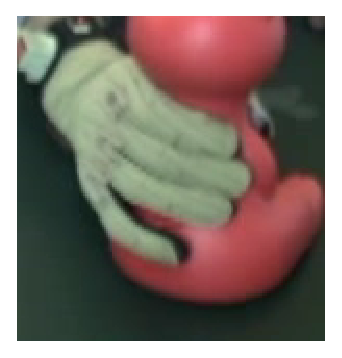
\includegraphics[width=0.19\textwidth]{images/cylinder}
%	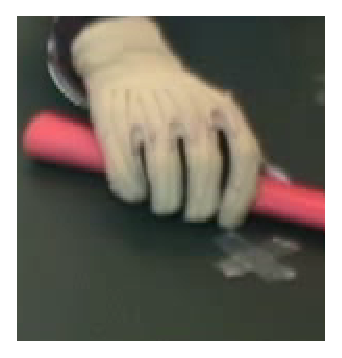
\includegraphics[width=0.19\textwidth]{images/flat}
%	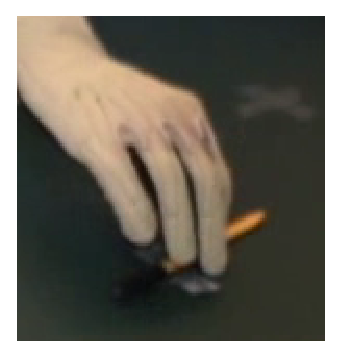
\includegraphics[width=0.19\textwidth]{images/pinch}
%	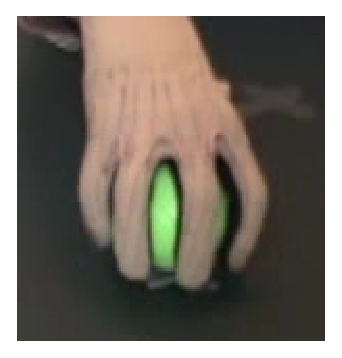
\includegraphics[width=0.19\textwidth]{images/spherical}
%	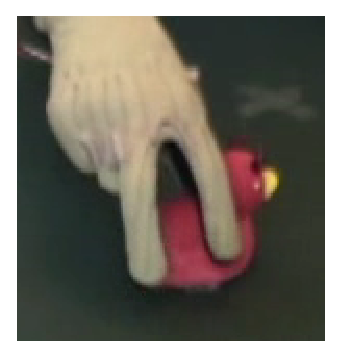
\includegraphics[width=0.19\textwidth]{images/tripodal}
%	\caption{The different grasping types that we consider: from left to rigth, {\it cylinder power}, {\it flat}, {\it pinch}, {\it spherical} and {\it tripodal} grasp.}
%	\label{fig::grasps}
%\end{figure}
%We consider 5 grasp classes, as shown in Fig. \ref{fig::grasps}, ideantified by different fingers poses.
%To summarize, the framework we have in mind should include components able to:
%\begin{itemize}
%	\item model and recognize an object
%	\item extract dynamic (visual and sensorial) information related to the action
%	\item estimate a regression model to obtain information on dynamic actions starting from knowledge about objects appearance.
%\end{itemize}
%This implementation leads us to obtain a system capable of [1] modelling the relation between objects and actions in terms of mapping between appropriate descriptions to handle the multimodality, and [2] predicting the suitable grasping action for a new instance of some known object in the test phase, where motion information are not available. The latter requirement can be thought of as the capability of estimating a {\it virtual grasp}.\\
%The system accepts in input a video signal showing object and dynamic of the action, so a natural choice lies in exploiting low-level measurements extracted from images to capture their appearance. Actions can be further described by means of sensors placed on hand and fingers, allowing to capture peculiarities typical of each grasping.\\
%In the remainder of the paper we will introduce the strategy adopted to implement the system modules and present the preliminary results giving evidence of the pertinence of the proposed approach to solve the problem of interest.


This section describes the visual and motor features used in our framework. We begin with the visual features 
(Section \ref{sec:vis-feat}) and then continue with the motor features (Section \ref{sec:mot-feat}).

\subsubsection{Visual Features}
\label{sec:vis-feat}

% \begin{figure}
% 	\centering
% 	\includegraphics[width=0.5\textwidth]{images/objects/SchemaVisionUnit.pdf}
% 	\caption{A schematic representation of how the visual features are extracted during training(left) and test(right).}
% 	\label{fig::vision}
% \end{figure}

The visual appearance of objects is captured by a dedicated item of the framework, %(see Figure \ref{fig::vision}), 
which
can be sketched as follows.
We first select from the video sequence a set of interesting frames where the object is clearly visible. 
To avoid contamination due to background elements, 
we apply change detection by comparing the selected frames against a background model, and then
restrict our attention on the region of interest (ROI) defined by the object bounding box.
We apply to the ROI a bag-of-keypoints object description \cite{csurka-dance-2004} designed as a two steps procedure \cite{ICIAP}:

\begin{itemize}

\item  We build the global vocabulary, by putting together keypoints extracted from images of all 
the objects into the dataset. As keypoints, we consider a set of randomly sampled points whose 
patch is modeled with a vector valued  descriptor which can be seen as a fixed scale SIFT  \cite{lowe}.
K-means is adopted to cluster the descriptors: the centroids 
(or virtual features) become the words of the visual vocabulary.

\item Both training and test images are thus represented with respect to the vocabulary, with a simple 
nearest neighbor approach.  At the end, visual appearance of objects is summarized with a frequency 
histogram, whose peaks should indicate which virtual features are the most important in modelling a specific object.

\end{itemize}

Notice that the vocabulary size is a system parameter which should be tuned with respect to the complexity of 
objects, to find a trade-off between sparsity of the descriptions and capability of characterizing the objects.           

Finally a remark is in order. From the point of view of appearance-based object recognition, %from visual cues
the experimental scenario is not challenging.
We opted for such a setting in order to keep the focus of the work on the joint modelling of visual and motor inputs.
% being the focus of the work instead to give 
%evidence of the fact that motion actually improves the recognition (classification) performances.

\subsubsection{Motor Features}
\label{sec:mot-feat}
The MPR are simply the $22$ angles returned by the dataglove, considered at
the time of contact of the subject's hand with the object\footnote{A
force-sensing resistor was used to determine the instant of contact.}. The
MPR is therefore a ``snapshot'' of the subject's hand in the instant of
grasping the object.


%\begin{figure}
%	\centering
%	\includegraphics[width=0.5\textwidth]{images/schema_vision.pdf}
%	\caption{A schema of the vision unit. First, suitable frames are extracted from the sequence and objects are located by means of background subtaction (BS). SIFT descriptors of a set of random points are input of a clustering step to get to the final visual vocabulary. Finally, each image is represented with respect to the vocabulary adopting a nearest neighbour (NN) strategy (see text for details).}
%	\label{fig::vision}
%\end{figure}

%As we will discuss in Sec. \ref{sec::experiments}, the system gathers, as one input, a video sequence acting as {\it spectator}, whose focus is on object appearance. The goal of the vision unit is to process the signal to obtain a global model of a set of given objects.
%Figure \ref{fig::vision} shows the pipeline of the vision unit when considering only one object (the same procedure is applied to the whole set of objects). Among the sequence, we first select the frames showing only the object  without any occlusion, then we locate more precisely its position by means of a simple background subtraction. 
%Although in our application there is not an explicit object recognition step, it is clear from the architecture pipeline that a robust and specific object model is functional to subsequent analysis. It is worthwhile also to mention that with the terms {\it object recognition} we indicate the characterization of a specific object instance (againts the concept of categorizing classes of objects).
%We adopt an approach based on local features to describe image structures: because of their popularity a rich variety of local measurements have been proposed in the literature \cite{harris,schmid,lowe} and applied successfully to objects recognition and categorization problems (see \cite{csurka,ferrari} just to name a few). 
%Local approaches tipically include two distinct steps: keypoints extraction and description. 
%However, in our case, a keypoint based-representation often ends up into a poor description
%due to the limited size of the images. We thus built our representation by extracting enough 
%random points  guaranteeing a more homogenous sampling.
%We chose to adopt SIFT descriptors \cite{lowe,schmid2} to model image patches around these points, obtaining a set of {\it words} for each image.\\
%To avoid redundancy and include some global information in our model, we apply k-means \cite{wong}, following the well-known bag-of-words approach \cite{csurka}. 
%We thus build a {\it global} vocabulary, containing SIFT descriptions of all known objects. 
%Image representation is obtained by means of frequency histogram of visual words, selecting for each random point extracted from the image 
%the most similar visual word as nearest neighbor. A normalization step may be advisable for the subsequent data processing.

%\textbf{Questa sezione non mi e' molto chiara....ma la perceptual representation non e'
%fatta da VPR e MPR? Perche' qui descriviamo solo la vision? 
%FEATURES
%---------
%-vision: SIFT, bag of words. 50 words vocabulary, image divided in 4 parts.
%Resulting in feature vectors with 200 elements. 
%-motor: The CyberGlove returns 22 8-bit numbers linearly related to the angles 
%of the subject's hand joints. Resulting in feature vectors with 22 elements.}


The VMM is supposed to be a regression strategy from visual to motor features, 
as defined above. Since the output is multivariate
(the motor features, consisting of $22$ numbers) and the input is very highly dimensional (the visual features, consisting of $200$
numbers), we decided
to enforce the VMM using neural networks. Each network was kept as
simple as possible: one hidden layer with $20$ neurons,
log-sigmoid transfer function and scaled conjugate gradient 
backpropagation. The training procedure used the early stopping
strategy, i.e. the training set was divided in a new training
and validation set. The network is evaluated on the validation set: 
when the performance stops improving, the algorithm halts. 

Most of these settings are inspired by the work of Richmond and others
\cite{papcun,richmond2007} on audio-to-motor mapping. In fact,
since each object may correspond to several grasps as it happens in reality
(recall the Section above), the relationship between the visual  and the motor features
is highly non-functional and it is in general hard, if not pointless, to
model it using a single NN. Richmond's idea was to model a \emph{probability
distribution} rather than a functional map; here we follow a somewhat more naive approach:
we define an ``archetipal grasp'' related to the specific
object observed. In the case of an object that can be grasped in only one way 
(for instance ``pig''), then the archetipal grasp will correspond 
to it. In case of an object graspable in different ways, then the 
archetipal grasp will correspond to an ``average'' grasp between those 
possible. We expect that this reconstructed grasp will have a 
positive effect on the overall performance of our object recognition system;
at the same time we hope that such representation won't get messed up
with other ones since the output space is also rather high-dimensional.


%The VMM Trying to map visual to motor information
%actually means defining a regression strategy. In our setting,
%we need a method which receive in input a SIFT feature vector
%and produces in output a sensorymotor feature vector. 
%A reasonable hypothesis is that every time we see an object 
%we are able to associate to it all the possible ways in
%which we know it can be grasped. The idea can be simplified
%supposing to define an ``archetipal grasp'',related to the specific
%object observed. In the case of an object that can be grasped in only one way 
%(for instance ``pig''), then the archetipal grasp will correspond 
%to it. In case of an object graspable in different ways, then the 
%archetipal grasp will correspond to an ``average'' grasp between those 
%possible. We expect that this reconstructed grasp will have a 
%positive effect on the overal performance of our object recognition system.
%
%We implemented this strategy using 7 neural
%networks, one for each object in the VMGdb database. All the
%neural networks are equal: 200 input values corresponding
%to the SIFT feature vector elements; 20 neurons in the hidden layer;
%22 output values corresponding to the sensorimotor feature vector 
%elemets; log-sigmoid transfer function; scaled conjugate gradient 
%backpropagation. The training procedure used the early stopping
%strategy, i.e. the training set was divided in a new training
%and validation set. The network is evaluated on the validation set: 
%when the performance stops improving, the algorithm halts. 
%
%\textbf{Solo qualche idea rozza: nella discussione finale andrebbe 
%detto che la rete neurale cosi' definita e' debole...la scelta del 
%numero nei neuroni nell'hidden layer e' 'occhiometrica': ...la teoria 
%suggerisce che dovrebbero essere di piu'...anche l'addestramento per ogni
%oggetto e' fatto usando circa 200 campioni, ma per come e' fatta la rete
%numero dei parametri che volgiamo stimare e' maggiore di 200...,
%avremmo bisogno di piu' campioni o diridurre la dimensione dei
%vettori di input ed output (sappiamo che non tutti gli elementi dei vettori
%SIFT e motor sono utili)}


\section{Experimental setup}
\label{sec::experiments}

The experimental phase aims at testing the proposed framework in a highly controlled environment, where we focus on learning the mapping between image descriptors and motor-sensor data to predict the grasp associated to each object. In the following we present the experimental setup and the regression results.

\subsection{Data acquisition setup}
\label{sec::acquisition}

Data were collected using two Watec \emph{WAT-202D} colour cameras for the images and a $22$-sensors Immersion \emph{CyberGlove} for the hand posture. An Ascension \emph{Flock-Of-Birds} magnetic tracker mounted on the subject's wrist, and a standard force sensing resistor glued to the subject's thumb were used to determine the hand position and speed, and the instant of contact with the object.\\
\begin{figure}[h!]
	\centering
	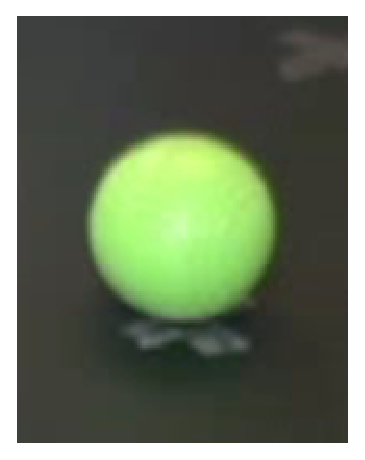
\includegraphics[height=1.75cm]{images/palla}
	
\includegraphics[height=1.75cm]{images/penna}
	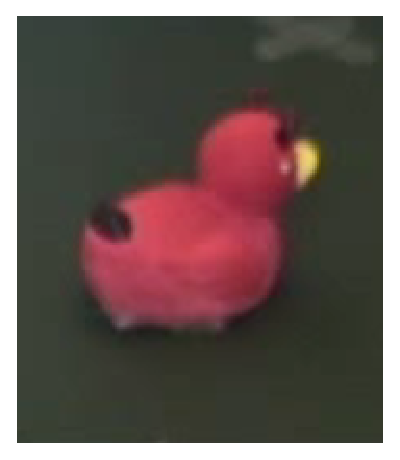
\includegraphics[height=1.75cm]{images/papera}
	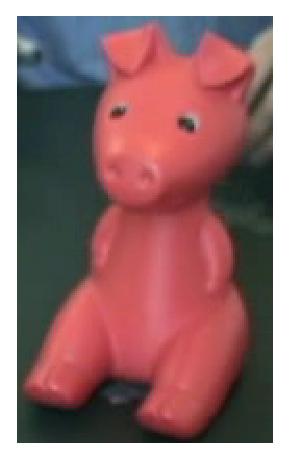
\includegraphics[height=1.75cm]{images/porcellino}
	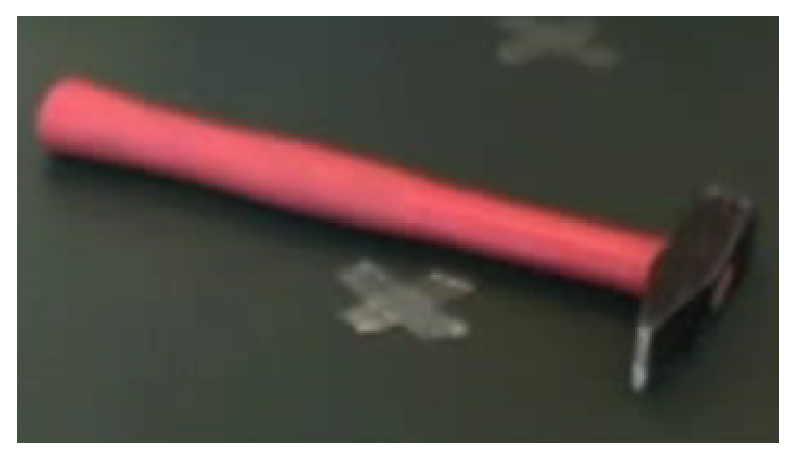
\includegraphics[height=1.75cm]{images/martello}
	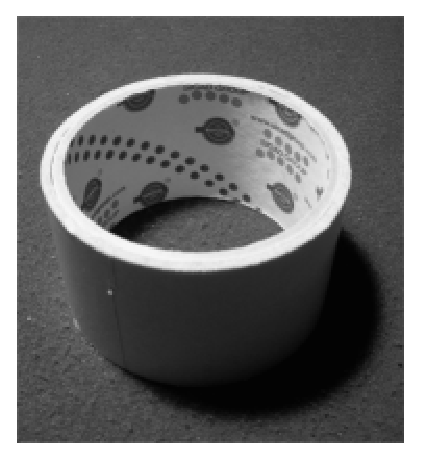
\includegraphics[height=1.75cm]{images/scotch}
	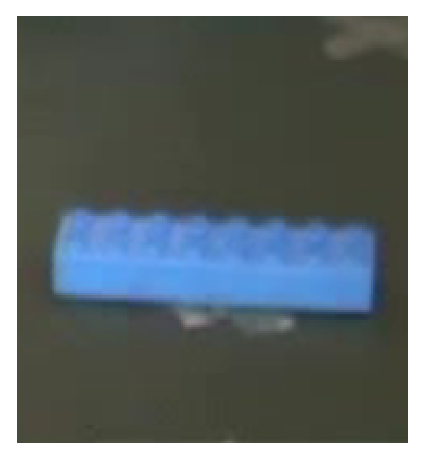
\includegraphics[height=1.75cm]{images/lego}\\
	\vskip 0.1cm
	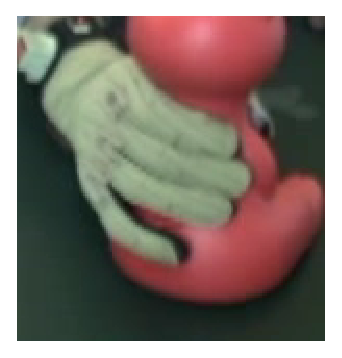
\includegraphics[width=0.19\textwidth]{images/cylinder}
	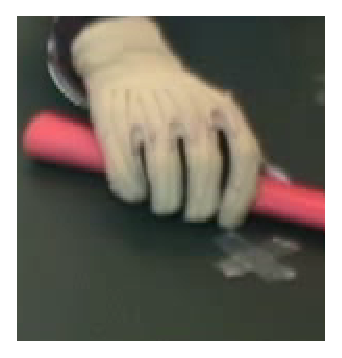
\includegraphics[width=0.19\textwidth]{images/flat}
	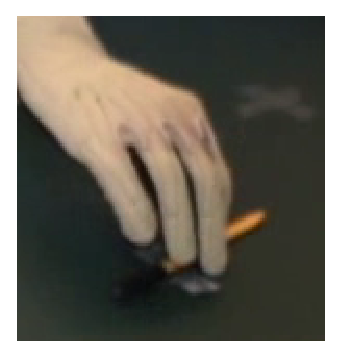
\includegraphics[width=0.19\textwidth]{images/pinch}
	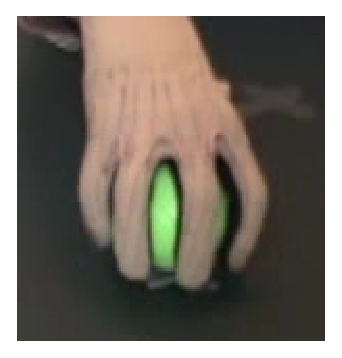
\includegraphics[width=0.19\textwidth]{images/spherical}
	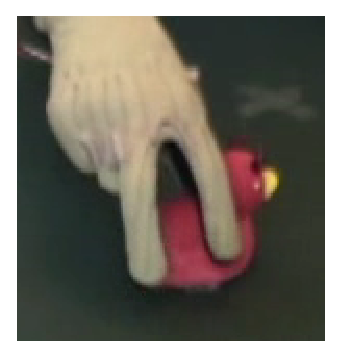
\includegraphics[width=0.19\textwidth]{images/tripodal}
	\caption{Top row: the objects used in our experiments. Bottom, the grasp types we consider: \emph{(left to right)} cylindric power grasp, flat grasp, pinch grip, spherical and
	tripodal grip.}
	\label{fig::grasps}
\end{figure}

The cameras return two video sequences, one placed laterally with focus on the object (the \emph{spectator}) and one placed in front of the subject (observing the \emph{actor}). We process only the {\em spectator} video sequence, because it supplies all the information required for preliminary testing. The video sequence is acquired at $25$Hz by each camera, while the glove is sampled at $100$Hz. Since the three devices are independent of one another a system of common time-stamps was used in order to synchronise the data.\\
The CyberGlove returns $22$ $8$-bit numbers linearly related to the angles of the subject's hand joints. The resolution of the sensors is on average about $0.5$ degree. The sensors describe the position of the three phalanxes of each finger
(for the thumb, rotation and two phalanxes), the four finger-to-finger
abductions, the palm arch, the wrist pitch and the wrist yaw.\\
For these preliminary experiments we considered $7$ objects and $5$ grasping types identified by different hand postures (see Fig. \ref{fig::grasps}); $2$ subjects have joined the experiment: for each object, the actor was asked to perform the required grasping action $20$ times. 

\subsection{Proof of concept experiments}
Among the motor data, it is reasonable to consider only the 22 measures of hand joints as the most relevant for accurately describing the intrinsic properties of each grasping type.
When a grasp occurs the pressure on the force sensing resistor increases, causing the signal to vary hence fixing the time-stamp 
of the event. Concurrently the values on each hand joint are stored as our output data.
%
%We select such data for interesting events (grasping actions) by analysing the signal of the pressure sensor, that assumes lower values when pressure increases.\\
By synchronising motor data and video sequence we select as input data the frames showing an object without clutter, going back along the sequence from the time-stamp in which the event occurs for a fixed amount of frames (see Fig. \ref{fig::vision}, left). 
Our data are thus generated as pairs of image descriptors and sensor-motor values, respectively input and output used to feed the regression model. %In the test phase only the visual information is available.\\ 
The regression methods discussed in Sec.\ref{sec::regression} are implemented in order to predict the expected sensor values of a grasp given the image of an object to be grasped. 
We compare four different image representations, based on bag-of-words descriptors where the histograms are computed for $20$ and $50$ words vocabularies on the entire image or on its four quadrants and then concatenated. We call the representations W20, W20conc, W50 and W50conc.\\
We consider two settings to evaluate the prediction performance of the proposed algorithms. In the first setting (V1-V2) we build training and test sets with the first and second volunteer's data respectively ($140$ examples each). In the second setting (MIXED) we mix the data of both volunteers and perform a 5 fold cross validation (5-CV). For both settings 5-CV on the training data only is used to select the regularizing paramenter for the RLS method and the stopping iteration for the Landweber and $\nu$-method. Tab.\ref{tab:results} summarizes the prediction errors evaluated according to the square loss on all $22$ components.
The prediction errors are consistent among the three learning methods, homogenous with respect to the setting and there are no significant differences among the four representations.
The values for the second setting are markedly lower because mixing the data of both volunteers reduces the variance between training and test sets in each split of the 5-CV. Therefore if we aim at building a model generalizing on several people, it is crucial to collect data from a large variety of volunteers.\\
\begin{table}[h!]
\centering
\begin{tabular}{|c|c|c|c|c|}
\hline Setting & Representation  & RLS $[10^3]$ & Land $[10^3]$ & Nu $[10^3]$\\\hline
\multirow{4}{*}{V1-V2} & W20conc  & $48$ & $47$& $47$\\\cline{2-5}
&W20  	  & $37$ & $38$& $38$\\\cline{2-5}
&W50conc & $41$ & $40$& $40$\\\cline{2-5}
&W50 	  & $43$ & $43$& $43$\\\hline
\multirow{4}{*}{MIXED} 
& W20conc & $6.1 (1.1) $ & $6.4 (1.2) $& $6.4 (1.2) $\\\cline{2-5}
& W20 & $7.9 (1.3) $ & $8.0 (1.2) $& $8.0 (1.3) $\\\cline{2-5}
&  W50conc &   $6.1 (0.8) $ & $6.1 (0.9) $& $6.3 (0.7) $\\\cline{2-5}
& W50 & $7.4 (2.0) $ & $7.2 (2.0) $& $7.3 (2.0) $\\\hline
\end{tabular}
\caption{Prediction accuracies of the proposed methods for the two settings and four representations. The accuracy is expressed as 
mean square error. In the MIXED scenario the associated variance is reported as well.}
\label{tab:results}
\end{table}
Finally, we aim at classifying the grasp type given the estimated sensor values.
We restrict at the MIXED setting, using the best regression outcome case,  W50conc/RLS.
The input data are the sensor measures and the output data are the grasp classes.
Again, a 5-CV is performed. For each split the training set is the actual set of measures from the sensors paired with the corresponding
grasp type, while the test set is the set of estimated measures.  
We train a RLS classifier \cite{rifkin03rlsc} in a One-vs-All configuration 
 obtaining a prediction accuracy of 99.6 (0.8)\%. 
 This result indicates that the regression models perform well and 
 guaranteeing the validity of the idea underlying the framework.











\section{Discussion and future work}
In this paper we proposed a general architecture for learning multi-modal patterns of data. 
The underlying assumption is that the system we want to model has several perceptual channels available, 
but among them some might be inactive. 
We adopted a regression-based approach to build a behavioral model of the system 
that can be exploited to amend such inactivity.
As a validation attempt, we presented an application for grasp prediction by means of vector 
valued regression: the experimental phase produced very promising results that encourage 
us to further investigate this framework. 
Even though the regression problem is inherently vector-valued, we  restricted 
our analysis to the simple scalar-valued case. 
A preliminary analysis on the covariance matrix of the sensors measures 
shows some correlation among the sensors, both positive and negative, 
pointing at the usefulness of a full-fledged vector-valued approach. 
Recently, much work has been devoted on how to best exploit the similarity among the components 
and learn all of them simultaneously. The main idea behind most of the literature is to use prior 
knowledge on the components relatedness to design a particular penalization term or a proper 
matrix-valued kernel \cite{micchelli04kernels}. 
In absence of prior knowledge, one approach is to design an heuristic to evaluate the similarity 
among the components from the available data, e.g. by computing the sample covariance of the 
sensor measures. 
Our current research is focused on how to translate this information into a viable matrix-valued kernel. 
Alternatively one can learn the vector structure directly in the training phase 
\cite{pontil08transferlearning,jacob08clusteredmtl}.  

This  multifaceted framework can be further extended in different directions. 
Regarding the experimental setup, we plan to enrich the dataset with a higher number of subjects, and multiple grasps for each object. Indeed, this will let us relax the one-to-one assumption we adopted in this paper and investigate a more realistic many-to-many mapping between objects and grasp classes.
As anticipated in the introduction, the modeled mapping will be used in the context of multimodal learning to investigate whether, by reconstructing a missing modality, the object recognition rate improves.
From the statistical learning viewpoint, we plan to explore new solutions drawing inspiration from the mentioned works on multitask learning. 

\subsection*{Acknowledgments}
This work was supported by the EMMA project sponsored by the Hasler Foundation (B. C.)

\begin{thebibliography}{4}

\bibitem{rizz} Rizzolatti, G., Craighero, L.: The Mirror-Neuron System. Annual Review of Neuroscience. 27:169-92 (2004)

\bibitem{harris} Harris, C., Stephens, M.: A Combined Corner and Edge Detector. Proceedings of The Fourth Alvey Vision Conference. pp. 147-151 (1988)

\bibitem{schmid} Mikolajczyk, K., Schmid, C.:Scale and Affine Invariant Interest Point Detectors. In IJC. V 60(1):63-86 (2004)

\bibitem{lowe} Lowe, D. G.: Distinctive Image Features from Scale-Invariant Keypoints. International Journal of Computer Vision. 60 (2): 91–110 (2004) 

%\bibitem{lindeberg} Lindeberg, T.: Feature Detection with Automatic Scale Selection. International Journal of Computer Vision. 30 (2): 79–116 (1998)

%\bibitem{perona} Moreels, P., Perona, P.: Evaluation of Features Detectors and Descriptors Based on 3D Objects. In ICCV. (2005)

\bibitem{schmid2} Mikolajczyk, K., Schmid, C.:A Performance Evaluation of Local Descriptors. Trans on PAMI. 27(10) (2005)

%\bibitem{leibe} Leibe, B., Mikolajczyk, K., Schiele, B.: Efficient Clustering and Matching for Object Class Recognition. In BMVC. (2006)

\bibitem{csurka} Csurka, G., Dance, C.R., Fan, L., Bray, C.: Visual Categorization with Bag of Keypoints. In ECCV. (2004)

\bibitem{ferrari} Ferrari, V., Tuytelaars, T., Van Gool, L.: Simultaneous Object Recognition and Segmentation from Single or Multiple Model Views. IJVC. 67(2) (2006)

\bibitem{LoGerfo08Spectral} Lo Gerfo, L., Rosasco, L., Odone, F., De Vito, E., Verri, A.:
  Spectral Algorithms for Supervised Learning. Neural Computation. 20(7) (2008)

 \bibitem{Yao07Early}
   Yao, Y., Rosasco, L., Caponnetto, A.: On Early Stopping in Gradient Descent Learning.
   Constructive Approximation. 26(2) (2007)

\bibitem{MicchPon05Onlearning} Micchelli, C.~A., Pontil, M.: On learning vector-valued functions.
  Neural Computation. 17 (2005)

\bibitem{dev04representer} De Vito, E., Rosasco, L., Caponnetto, A., Piana, M.,	Verri, A.:Some Properties of Regularized Kernel Methods. Journal of Machine Learning Research. 5 (2004)

\bibitem{preprint} Baldassarre, L., Barla, A.,  Rosasco, L., Verri, A.:
Learning vector valued functions with spectral regularization. (preprint)

% \bibitem{jung} Hye-Won, J., Yong-Ho, S., Ryoo, M.S., Yang, H.S: Affective Communication System with Multimodality for a Humanoid Robot, AMI.
% 4th IEEE/RAS International Conference on Humanoid Robots. 2 (2004)

% \bibitem{kruger} Kr$\ddot{u}$ger, N., Felsberg, M., W$\ddot{o}$rg$\ddot{o}$tter, F.: Processing Multi-modal Primitives from Image Sequences. 4th ICSE Symposium on Engineering of Intelligent Systems. (2004) 

% \bibitem{yang} Yang, G., Lin, Y., Bhattacharya, P.: Multimodality Inferring of Human Cognitive States Based on Integration of Neuro-Fuzzy Network and Information Fusion Techniques. EURASIP Journal on Advances in Signal Processing. 8(2008)

\bibitem{gallese} Gallese, V., Fadiga, L., Fogassi, L., Rizzolatti, G.: Action Recognition in the Premotor Cortex. Brain. 119, 593–609 (1996)

% \bibitem{grans} Granström, B. House, D., Karlsson, I.: Multimodality in Language and Speech Systems. Text, Speech and Language Technology. 19(2002)

\bibitem{metta} Metta, G., Sandini, G., Natale, L., Craighero, L., Fadiga, L.: Understanding  Mirror Neurons: A Bio-Robotic Approach. Interaction Studies. 7, 197–232, (2006)

% \bibitem{caputo} Luo, J., Pronobis, A., Caputo, B.: SVM-based Transfer of Visual Knowledge Across Robotic Platforms. 5th International Conference on Computer Vision Systems. (2007)

% \bibitem{thrun} Thrun, S., Mitchell, T.: Lifelong Robot Learning. Robotics and Autonomoues Systems. 15 (1995)

% \bibitem{malak} Malak, R.J., Khosla, P.K.: A Framework for the Adaptive Trasfer of Robot Skill Knowledge Using Reinforcement Laerning Agents. Proc of ICRA. (2001)

% \bibitem{barto} Konidaris, G., Barto, A.G.: Autonomous Shaping: Knowledge Transfer in Reinforcement Learning. Proc. of ICML. (2006) 

\bibitem{wong} Hartigan, J. A., Wong, M. A.: A K-Means Clustering Algorithm". Applied Statistics. 28(1) (1979) 

\bibitem{cutkosky} Cutkosky, M.: On grasp choice, grasp models and the design of hands for manufacturing tasks. IEEE Transactions on Robotics and
Automation. (1989)

\bibitem{2007.AR} Castellini, C., Orabona, F., Metta, G., Sandini, G.: Internal Models of Reaching and Grasping. Advanced Robotics. 21(13) (2007)

%\bibitem{papcun} Papcun, G., Hochberg, J., Thomas, T. R., Laroche, F., Zacks, J., Levy, S.: Inferring articulation and recognizing gestures from acoustics with a neural network trained on x-ray microbeam data. J Acoust Soc Am. 92(2) (1992)

%\bibitem{richmond} Richmond, K., King, S., Taylor, P.: Modelling the uncertainty in recovering articulation from acoustics. Computer Speech and Language. 17 (2003)

\bibitem{bulmann02boosting} Buhlmann, P.: Boosting for High-Dimensional Linear Models". Annals of Statistics. 34(2), 559–58 (2006)

\bibitem{micchelli04kernels} Micchelli, C. A., Pontil, M.: Kernels for Multi-task Learning. NIPS (2004)

\bibitem{rifkin03rlsc} Rifkin, R., Yeo, G., Poggio, T.: Regularized Least-Squares Classification. Advances in Learning Theory: Methods, Models and Applications. (2003) 

\bibitem{pontil08transferlearning} Argyriou, A., Maurer, A., Pontil, M.: An Algorithm for Transfer Learning in a Heterogeneous Environment. ECML/PKDD. (1) 71-85 (2008) 

\bibitem{jacob08clusteredmtl} Jacob, L., Bach, F., Vert, J.P.: Clustered Multi-Task Learning: a Convex Formulation. NIPS. (2008) 

\end{thebibliography}

\end{document}
